% Source: graduate-coursework/Sp26/CSCE775/course_notes/practice_problems.tex

\documentclass[border=4pt]{standalone}
\usepackage{amsmath, amssymb, amsthm}
\usepackage{tikz}
\usepackage{xcolor}
\usetikzlibrary{arrows.meta, positioning, shapes.geometric}

\definecolor{Garnet}{RGB}{115, 0, 10}
\definecolor{Atlantic}{RGB}{70, 106, 159}
\definecolor{Congaree}{RGB}{31, 65, 77}
\definecolor{NinetyBlack}{RGB}{54, 54, 54}
\definecolor{FiftyBlack}{RGB}{162, 162, 162}

\begin{document}
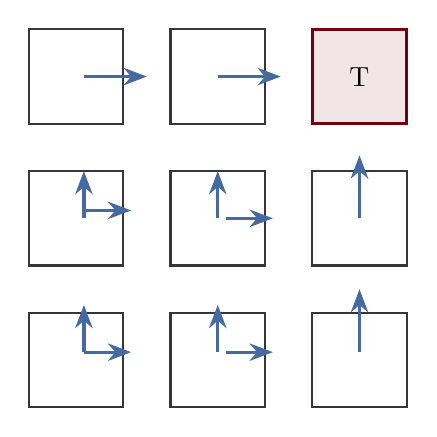
\begin{tikzpicture}[
    cell/.style={rectangle, minimum size=1.2cm, draw=NinetyBlack, thick},
    terminal/.style={rectangle, minimum size=1.2cm, draw=Garnet, very thick, fill=Garnet!10},
    arrow/.style={-Stealth, very thick, Atlantic}
]

% Grid cells
\foreach \row in {0,1,2} {
    \foreach \col in {0,1,2} {
        \ifnum\row=2
            \ifnum\col=2
                \node[terminal] at (\col*1.8, \row*1.8) {T};
            \else
                \node[cell] at (\col*1.8, \row*1.8) {};
            \fi
        \else
            \node[cell] at (\col*1.8, \row*1.8) {};
        \fi
    }
}

% Arrows showing greedy policy
% (0,0): Up or Right
\draw[arrow] (0.1, 0.1) -- (0.1, 0.7);
\draw[arrow] (0.1, 0.1) -- (0.7, 0.1);

% (0,1): Up or Right
\draw[arrow] (1.8, 0.1) -- (1.8, 0.7);
\draw[arrow] (1.9, 0.1) -- (2.5, 0.1);

% (0,2): Up
\draw[arrow] (3.6, 0.1) -- (3.6, 0.9);

% (1,0): Up or Right
\draw[arrow] (0.1, 1.8) -- (0.1, 2.4);
\draw[arrow] (0.1, 1.9) -- (0.7, 1.9);

% (1,1): Up or Right
\draw[arrow] (1.8, 1.8) -- (1.8, 2.4);
\draw[arrow] (1.9, 1.8) -- (2.5, 1.8);

% (1,2): Up
\draw[arrow] (3.6, 1.8) -- (3.6, 2.6);

% (2,0): Right
\draw[arrow] (0.1, 3.6) -- (0.9, 3.6);

% (2,1): Right
\draw[arrow] (1.8, 3.6) -- (2.6, 3.6);

\end{tikzpicture}
\end{document}
